%.-------------------------------------------------------------------------------------------------------------------------------------------------------------
\subsection{Product perspective}
The system will be developed from scratch using external elements such as Mapping systems and algorithm to recognise licence plates. We choose to take those external elements to decouple mapping problems from our project implementation and to use already tested algorithms to recognise licence plates.

%.-------------------------------------------------------------------------------------------------------------------------------------------------------------
\subsubsection{Class Diagram}
\begin{figure}[h]
\centering
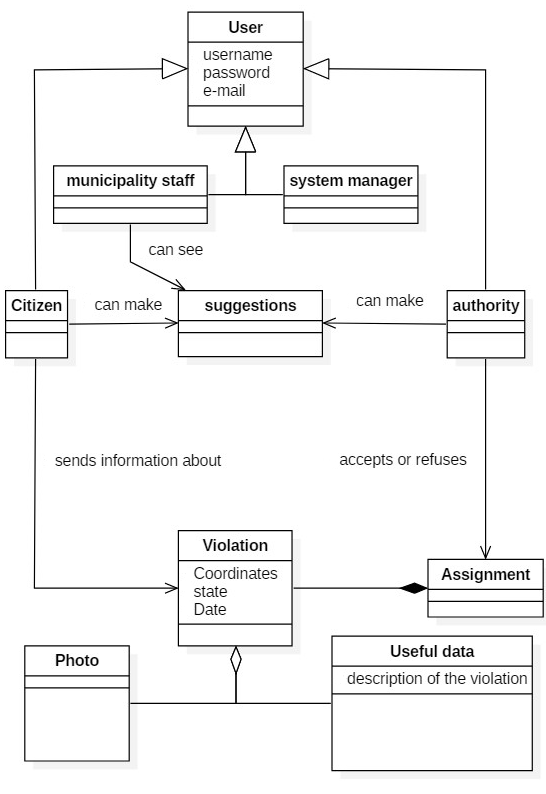
\includegraphics{Images/classdiagram.png}
\caption{\label{fig:cs} Class Diagram}
\end{figure}
\newpage
%.-------------------------------------------------------------------------------------------------------------------------------------------------------------
\subsubsection{Statechart report}
\begin{figure}[h]
\centering
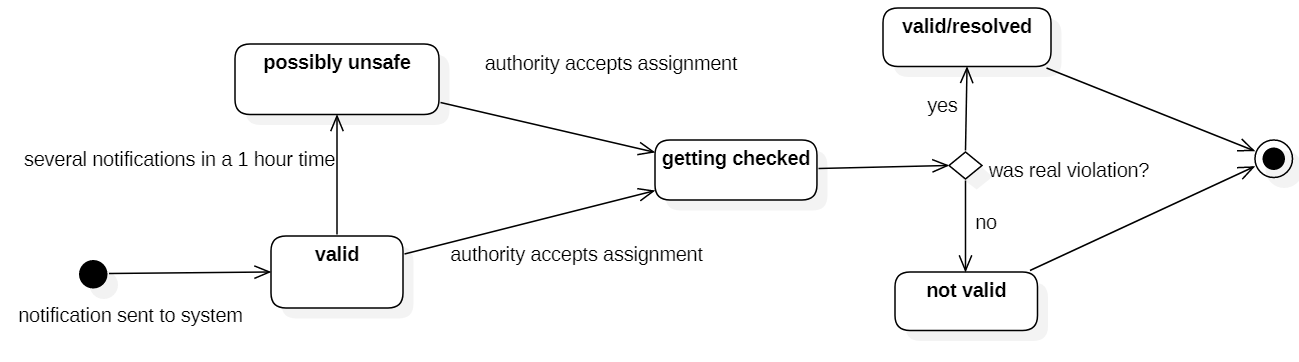
\includegraphics[width=\textwidth]{Images/statechartreport.png}
\caption{\label{fig:sc1} Statechart report}
\end{figure}
%.-------------------------------------------------------------------------------------------------------------------------------------------------------------
\subsubsection{Statechart assignment}
\begin{figure}[h]
\centering
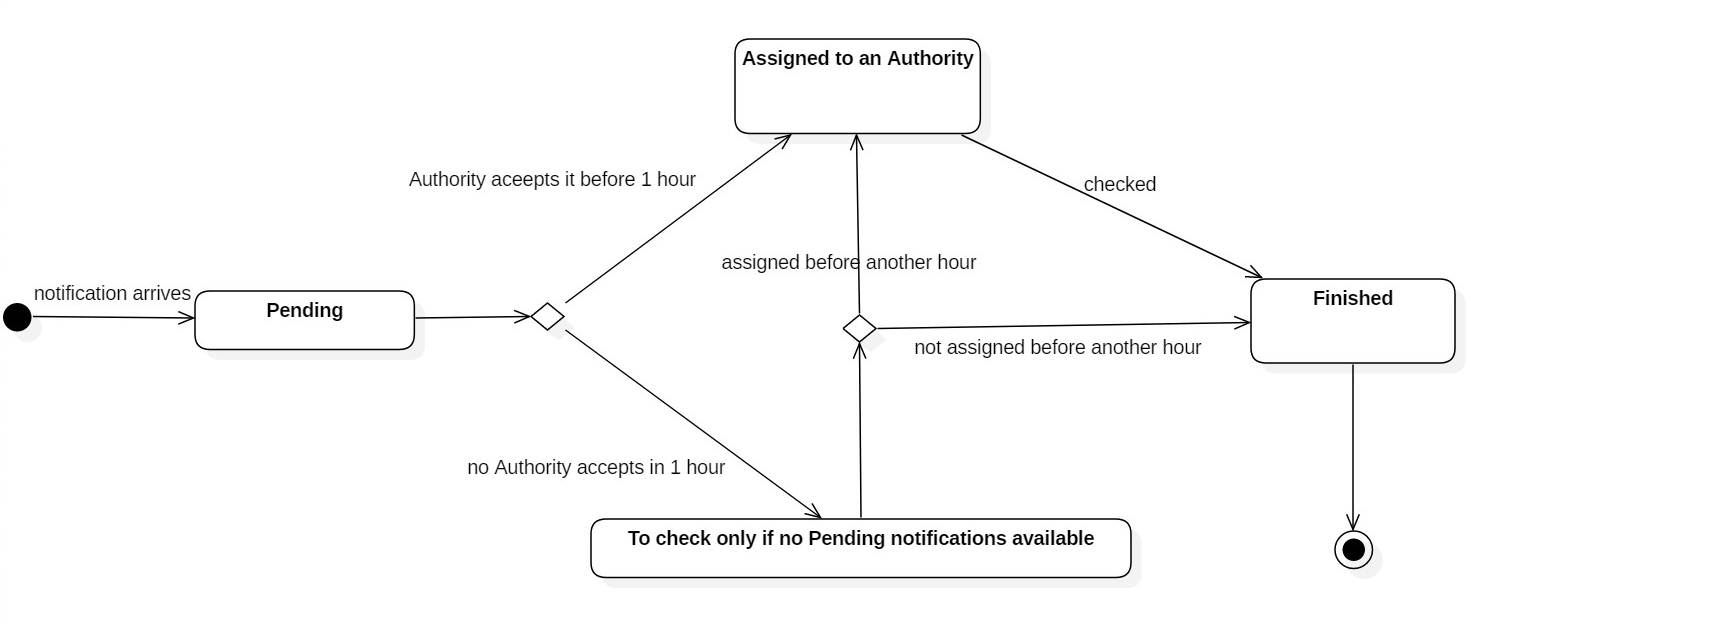
\includegraphics[width=\textwidth]{Images/statechartassignment.png}
\caption{\label{fig:sc2} StateChart assignment}
\end{figure}



%.-------------------------------------------------------------------------------------------------------------------------------------------------------------
\subsection{Product functions}
In this section we provide a list of functionalities offered by our system. We will describe those functionalities and in later section we will better analyse interactions of users with those functions.
%.-------------------------------------------------------------------------------------------------------------------------------------------------------------
\subsubsection{ Mapping System }
An external mapping system will be used to guarantee better performances than a system implemented from scratch.
This won’t always ensure the correctness of information given by that system. Some issues about mapping systems like accidents occurred and blocked streets can’t be addressed in real time. Those kinds of problems may need to rely on authority’s knowledge of the area to be overcome.
%.-------------------------------------------------------------------------------------------------------------------------------------------------------------
\subsubsection{Licence Plate Recognition Algorithm}
An external Licence Plate recognition algorithm will be adopted in our system. Online there are a lot of services and some open-source solutions. Those systems are used by several people and companies and have already been tested, so most kind of issues that may occur have already been noticed and fixed. Considering our system is to be launched in Italy we will consider a solution better suited to recognize European licence plates.
%.-------------------------------------------------------------------------------------------------------------------------------------------------------------
\subsubsection{Municipality Servers maintenance}
Our system can’t address municipality server’s unavailability issues. If a server is unavailable and needs maintenance, statistics for the area covered by that server may become unavailable for an indefinite amount of time. In order to solve this problem, SafeStreets may use the email address used to register the municipality to contact it and to point out the issues.
%.-------------------------------------------------------------------------------------------------------------------------------------------------------------
\subsection{Actors characteristics}
\begin{itemize}
\item Visitor: a person using SafeStreets without being registered. He/she can only see statics, register or sign-in to be recognized as a User
\item Registered User/ User: term used to identify any person which uses our application and has registered to our service:
\item  Citizen: Is a User who provide information to the system and is the main contributor to the service.
He/she provides information about violations with photos and possibly some notes. He/she can access data gathered by the system in form of statistics.
\item Municipality: Users managing local systems in each area. Those users should be able to take decisions to change unsafe areas thanks to their status.
\item Authority: police agents. They are invited to use the service by municipality users who can create their account. They can reserve assignments of violations to be addressed. They can also refuse the assignment, mark it as spam or send it to another authority.
\item System Manager: User who is responsible of the system, therefore he/she has all the possible privileges to manage the system.For example he/she can register a new municipality
\end{itemize}
%.-------------------------------------------------------------------------------------------------------------------------------------------------------------
\subsection{Assumptions, dependencies and constraints}
%.-------------------------------------------------------------------------------------------------------------------------------------------------------------
\subsubsection {Regulatory policies}
The system will ask user for minimal information to recognize them. The visitor should give the system only his /her email address and provide the system a username and a password to create an account. Email addresses won’t be used for commercial uses and will be stored only to give the possibility to recover an account in case the user loses his/her credentials.
%.-------------------------------------------------------------------------------------------------------------------------------------------------------------
\subsubsection{ Interfaces to other applications}
In the first release no public interfaces will be opened and SafeStreets will only communicate with municipality servers to retrieve useful information about accidents.
%.-------------------------------------------------------------------------------------------------------------------------------------------------------------
\subsubsection{ Domain assumptions}
\begin{itemize}
\item D1) For each notification data and metadata about the violation are correct
\item D2) Each Username is unique
\item D3) Authorities always intervene in case of a notified violation
\item D4) Information about authorities’ location are always available through GPS 
\item D5) Only agents close to the violation area are notified 
\item D6) Citizen sends only clear photos (if it is not clear he/she would retake the photo)
\item D7) System Manager, Municipality and authorities respects their duty of care
\item D8) When an authority is sent an email to register this will surely be received
\item D9) Information provided by authority are correct and no false report is ignored (always reported by authority as false).
\item D10) Citizens’ Location are retrieved by GPS or manual input and are correct
\item D11) The Agent must be contactable from municipality  
\item D12) Information of authority are known by municipality
\item D13) Information provided from Users must be correct
\end{itemize}
